\chapter{Introdução}
\label{chap:introducao}

A ordem de Hexabytes em dados estão disponíveis para análise em organizações, hoje em dia, através de informações provenientes de bases internas e externas \cite{google}, \cite{bing}. Estas enfrentam vários desafios quando tentam analisar dados gerados com o objetivo de extrair informações úteis \cite{Wu2008}, \cite{Mitsa:2010}, \cite{cheng:2014}, \cite{Atluri:2018}.

Esta capacidade analítica é possível por meio de ferramentas capazes de lidar com os dados sem tornar o processo de análise uma tarefa árdua. Os agrupamentos de dados normalmente são usados no processo de análise de dados, devido esta técnica não exigir qualquer conhecimento prévio, apesar dos algoritmos de agrupamento, dentre eles o dinâmico, geralmente, requerem um ou mais parâmetros de entrada, que influenciam o processo de agrupamento e os resultados que podem ser obtidos. 

Motos, táxis e caminhões, que instalam receptores de sistema de posicionamento global (\acrshort{GPS} - \emph{\acrlong{GPS}}), podem ser monitorados no estado de execução, cujos registros dessas informações espaciais e temporais são armazenados a cada segundo. Toda essa informação espaço-temporal é útil para a análise de padrões no espaço e no tempo. O espaço pode ser representado por um endereço, coordenadas geográficas de latitudes e longitudes, ou coordenadas locais (X, Y). O tempo pode ser exibido por ano, mês e dia e, às vezes, com detalhes como hora, minuto ou segundo \cite{Zhicheng:2019}.


O processo de agrupamento de dados ganhou uso muito difundido, especialmente para dados estáticos. No entanto, o rápido crescimento da demanda por informações espaço-temporais de inúmeros instrumentos e processos: como os satélites em órbita terrestre, acompanhamento das mudanças climáticas, ocorrências das mais diversas, trânsito nas cidades, dentre outros, criaram uma necessidade de métodos de agrupamento espaço-temporais para extrair e monitorar agrupamentos dinâmicos. Os conjuntos de dados coletados, independentemente de estarem em forma de tabela ou gráfico, são muitas vezes complexos demais para serem entendidos. Diante disso, métodos eficiente de análise espaço-temporal são importantes para determinar padrões significativos para melhor compreensão ou visualização \cite{Shekhar2011}.

Nos últimos anos, o problema de agrupamento dinâmico tem atraído o interesse de pesquisas, impulsionado pelo aumento da disponibilidade de grandes conjuntos de dados, contendo elementos espaciais e temporais. Este problema pode ser analisado como um problema de otimização, ou de particionamento. Seu objetivo principal é maximizar as diferenças das características dos indivíduos de grupos distintos, e minimizar as diferenças das características dos indivíduos de um mesmo grupo. O agrupamento espaço-temporal dinâmico considera que os individuos se movimentam no espaço e no tempo atualizando, inclusive, suas características individuais. Deste modo, este processo enfrenta dois grandes desafios no seu reconhecimento: primeiro, os grupos (\textit{clusters}) que são dinâmicos podem mudar de tamanho, forma e propriedades estatísticas ao longo do tempo e mesmo no espaço. Em segundo lugar, vários dados espaço-temporais são incompletos, ruidosos, heterogêneos e altamente variáveis no espaço e tempo. O problema de agrupamento dinâmico é encontrar grupos de dados de máxima dissimilaridade que evoluem no tempo e no maior tempo possível (ou com a maior estabilidade possível). Já o problema de previsão de grupos dinâmicos introduz o conceito de indicar os possíveis grupos que serão formados no tempo após um conjunto de eventos serem observados previamente.

Métodos de previsão de agrupamentos dinâmicos têm sido estudados nas áreas de climatologia, detecção de doenças, entre outras. Estes estudos concentram-se em modelos espaço-temporais que indicam caminhos de solução baseados na densidade espaço-temporal dos dados \cite{gupta:2014}. 

No Brasil, o problema da expansão e contração das doenças provocadas por Arboviroses é imenso, pois afeta centenas de milhares de pessoas ano a ano. Os sistemas de controle das doenças provocadas pelo \emph{Aedes Aegypti}, tais como a dengue e chikungunya, têm sido bastante negligenciados, apesar de muitos esforços isolados neste sentido: TabWin \cite{tabwin}, MonitoraDengue \cite{monitoraDengue}, \acrshort{SISPNCD} \cite{fad}, \acrshort{SUCEN} \cite{sucen} e \acrshort{LAIS} \cite{laisrn}.

Como os esforços e a informação são desagregados, o gerenciamento do processo de prevenção e controle ainda é muito difícil, tornando ineficiente o trabalho de campo, haja vista as poucas facilidades de coordenação, pessoal, recursos de mobilidade e projeção em tempo real dos acontecimentos.

Até onde se sabe, poucas ou nenhuma das ferramentas indicadas são capazes de integrar os diferentes esforços em um único arcabouço computacional que permita fazer o processo de gestão das diversas frentes da prevenção e controle de arboviroses. Os esforços realizados pelo Laboratório de Inovação Tecnológica em Saúde (LAIS) com o software \emph{Observatório do AEDES} da Universidade Federal do Rio Grande do Norte opera com georreferenciamento de focos de dengue por denúncia voluntária, usando \emph{smartphones}, e possui um aplicativo para acompanhamento de visitas de agentes da vigilância sanitária no campo. Relatórios e visualizações georreferenciadas são resultantes daí. Com o SUCEN da Secretaria de Saúde do Estado de São Paulo, são disponibilizadas na web facilidades para se dar entrada nos dados de monitoramento de todos os municípios com todos os endereços tabulados a partir do TABWIN. Também é possível gerar mapas temáticos e fazer várias consultas específicas, e criar os próprios mapas de consultas. Rotas de agentes são estáticas, e não se contempla o controle de pontos estratégicos. Há um sistema para \emph{tablet}, que acompanha os agentes sanitaristas em campo. Estas ferramentas mostram porém que podem ser integradas de modo a usar recursos móveis, porém modelos de gestão logística com Pesquisa Operacional ainda não são usados. 

\citeautoronline{webdengue2011} propuseram o arcabouço computacional WebDengue, que integra através de uma plataforma web com parcelas em \emph{desktop} e \emph{smartphones}, todas as ações em sistemas próprios para o planejamento e controle logístico de visitas de agentes de endemias, planejamento / acompanhamento / notificação / eliminação da presença do vetor em campo, acompanhamento e notificação de casos humanos e transmissão de informação entre laboratórios de zoonoses, para identificação dos Artrópodes e laboratório central de análises clínicas da presença dos vírus e patologia \acrshort{LACEN}, exibido na figura \ref{fig:webdengue}.

O principal objetivo do \citeautoronline{webdengue2011} era de mapear a evolução da dengue na cidade de Fortaleza, tomando como base as características de evolução dos casos e focos da doença observados em 2005 para a Regional II de Fortaleza-CE. A pesquisa se preocupou em definir intervalos de observação que justificassem um comportamento de evolução do mosquito \emph{Aedes Aegypti} e dos casos humanos da doença. O \textit{framework} WebDengue \cite{webdengue2008}, possui uma estrutura computacional que se constitui numa solução de vigilância epidemiológica composta por um conjunto de sistemas computacionais. Essas tecnologias combinam geoprocessamento, sistemas de apoio a decisão, sistemas de bancos de dados e a aquisição de dados remotos. Agora incorpora um poderoso Armazém de Dados (\acrshort{DW} - \textit{\acrlong{DW}}) para fazer previsões dos locais onde ocorrerão a doença.

\begin{figure}[!ht]
	\centering
	\Caption{\label{fig:webdengue} Estrutura computacional proposta para a gestão da dengue}	
	\UECEfig{}{
		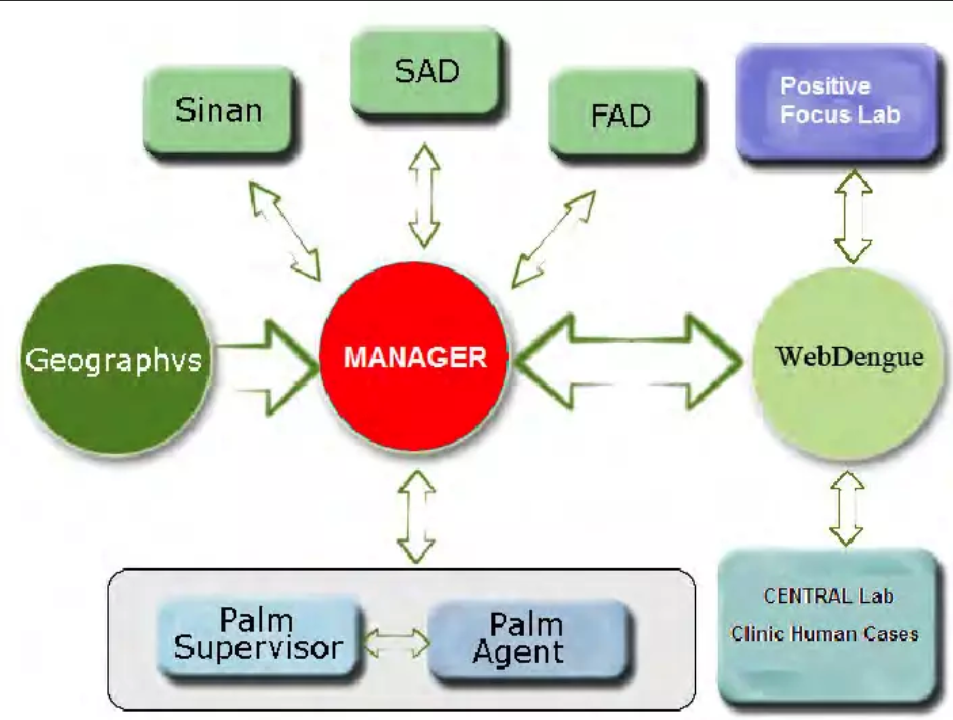
\includegraphics[width=12cm]{figuras/webdengue.png}
	}{
		\Fonte{Sistema WebDengue \cite{webdengue2011} }
	}
\end{figure}

O WebDengue \cite{webdengue2011}, possui nativamente uma base de dados organizada em um Banco de Dados espaço-temporal, que permite aos gestores realizarem diversas avaliações analíticas, de modo que se possa obter o melhor resultado no tratamento epidemiológico das arboviroses. Modelos estatísticos de previsão usando técnicas padrão (Médias Móveis, suavização exponencial, \emph{holt-winters} e outras), fazem parte do \emph{framework}. Apesar disto, notou-se que tais modelos não ajudam muito no processo de acompanhamento da dinâmica da expansão das arboviroses, pois não identificam nos bairros as áreas mais afetadas e que devem ser trabalhadas pelos agentes no sentido de debelar tais doenças.

A tarefa de agrupamento depende muito das características específicas dos dados e a maneira como eles são relacionadas. A Figura \ref{fig:st-types} exibe uma possível classificação de tais tipos de dados, com base na dimensão temporal, que descreve em que medida a evolução do objeto é capturada pelos dados, e a dimensão espacial, que descreve se os objetos estão associados a um local fixo ou sua localização é dinâmica e pode mudar no tempo.
Os tipos de dados espaço-temporais podem ser divididos em cinco categorias contendo eventos, variáveis georreferenciadas, séries temporais georreferenciadas, pontos em movimento e trajetórias. \citeautoronline{Kisilevich2009} descrevem as principais classes de tipos de dados:

\begin{figure}[!ht]
	\centering
	\Caption{\label{fig:st-types} Contexto para agrupamento espaço-temporal}	
	\UECEfig{}{
		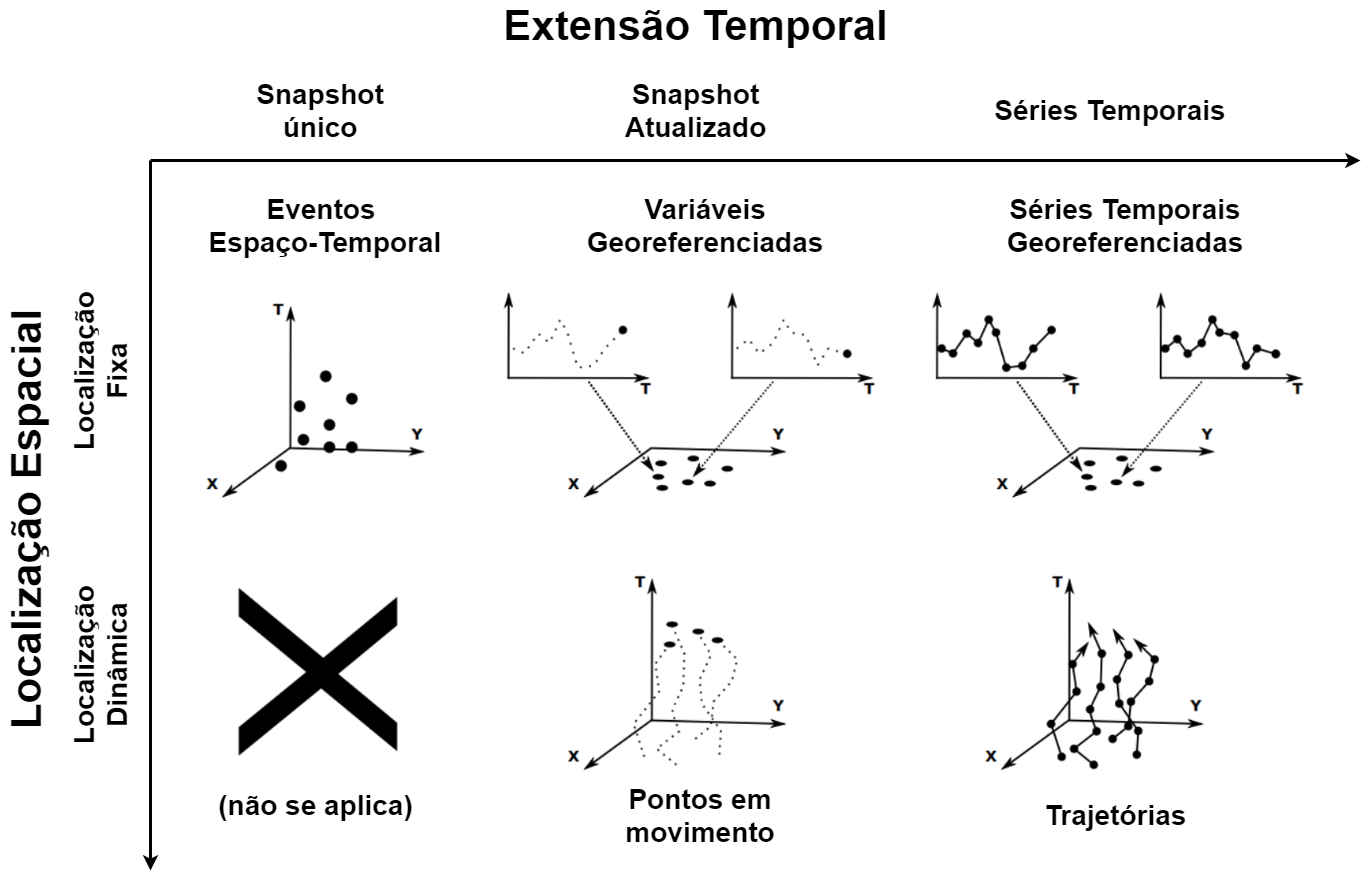
\includegraphics[width=15cm]{figuras/st-tipos.png}
	}{
		\Fonte{Elaborado pelo autor baseado em \cite{Kisilevich2009}}
	}
\end{figure}

\begin{itemize}
    \item Eventos Espaço-temporal: Um exemplo básico de informação espaço-temporal são os eventos espaço-temporais, como registros georreferenciados de uma epidemia. Cada evento é geralmente associado ao local onde foi registrado e ao registro de data e hora correspondente. Tanto a informação espacial quanto a temporal associada aos eventos são estáticas, uma vez que nenhum movimento ou qualquer outro tipo de evolução é possível. Encontrar grupos entre eventos significa descobrir que estão próximos no tempo e no espaço e possivelmente compartilham outras propriedades não espaciais. \citeautoronline{Birant2007STDBSCANAA} propuseram o algoritmo de agrupamento espaço-temporal \acrshort{ST-DBSCAN} que é uma extensão do algoritmo DBSCAN. Outro algoritmo para agrupamento espaço-temporal é o ST-IGN que é uma extensão do algoritmo IGN \cite{ign}. Esses dois algoritmos de agrupamento espaço-temporais foram implementados nesta dissertação para consolidar a metodologia proposta.
	\item Variáveis Georreferenciadas: quando é possível observar a evolução no tempo de alguns fenômenos em um local fixo, tem-se o que normalmente é chamado de uma variável georreferenciada, ou seja, o valor de mudança de tempo de alguma propriedade observada.
	\item Séries temporais georreferenciada: pode ser possível armazenar todo o histórico do objeto em evolução, fornecendo, portanto, uma série temporal (georreferenciada) para as variáveis medidas. Quando muitas variáveis estão disponíveis, elas geralmente são vistas como uma única série temporal multidimensional. Nesse caso, agrupando um conjunto de objetos requer comparar a maneira como a série temporal evolui e relacioná-la à sua posição espacial.
	\item Pontos em movimento: quando a localização espacial do objeto de dados está mudando no tempo. No caso mais simples, as informações disponíveis sobre esses objetos consistem em sua posição mais recente, como no contexto de monitoramento em tempo real de veículos.
	\item Trajetórias: descrevem o comportamento de movimento dos objetos e, portanto, o agrupamento pode ser usado para detectar grupos de objetos que se comportam de maneira semelhante.
\end{itemize}

Motivados pelo problema, o grupo de pesquisa em \textit{Data Mining e Categorização de Informações em Larga Escala}, desenvolveu uma concepção genérica de esforços no sentido de permitir a geração de modelos de previsão espaço-temporais da ocorrência de doenças provocadas por arbovisores. O primeiro passo nesse sentido foi dado com a criação de um modelo de visualização espaço-temporal robusto, denominado \emph{Dynagraph} \cite{dynagraph}, e o segundo seria a concepção, análise, implementação e avaliação de resultados de um \acrfull{SAD} que permita reconhecer agrupamentos de casos humanos de arboviroses, já que o mosquito se manifesta em concentrações definidas nas áreas urbanas de alta sucetibilidade à sua sobrevivência \cite{comportamentoDengue}.
Esta dissertação estuda o comportamento de métodos de agrupamento dinâmico espaço-temporais, considerando uma aplicação no monitoramento do avanço dos casos humanos de doenças provocadas por arboviroses (dengue e chikungunya) em Fortaleza/CE.

A representação dinâmica dos eventos também tem sido um problema importante. Muitos modelos são utilizados tais como representação espaço-temporal por vídeos e grafos. Na representação espaço-temporal por vídeos, o objetivo é sincronizar os modelos de previsão com a descoberta dos agrupamentos enquanto um vídeo real acontece (usado principalmente na climatologia \cite{faghmous2013}); já a representação dinâmica por grafos dinâmicos, tem sido estudada pela literatura com maior profundidade pois permite acompanhar eventos e gerar previsões espaço-temporais sabendo-se e controlando-se os principais atores do processo, tais como: elemento dinâmico e contexto dinâmico como descritos em \cite{holme:predictability} e \cite{Mitsa:2010}.

Ferramentas de grafos dinâmicos foram desenvolvidas e seguem em uso, como o Gephi \cite{gephi} e o Dynagraph \cite{dynagraph}. Aqui será feito um trabalho sobre o modelo Dynagraph para representação de uma estrutura dinâmica incluindo a possibilidade de variação dinâmica das características (cor, forma, tamanho, etc) dos elementos do grafo. Deste modo, esta visão evolutiva ajudaria ao modelo sistêmico representar claramente a realidade da evolução dos fenômenos que se deseja demonstrar para facilitar a tomada de decisão.

O problema básico de decisão associado a esta dissertação pode ser enunciado do seguinte modo: \emph{Considere-se que são dados grupos de indivíduos que ocupam áreas espaciais de uma determinada região e que ocorrem em um certo período de tempo. Deseja-se posicionar um conjunto mínimo de círculos (alvos), cujas áreas são mínimas, mas que também maximizam a cobertura dos grupos dados.} É pressuposto que tais círculos também maximizam a probabilidade de ocorrência de novos indivíduos nas áreas dos alvos definidos.

\section{Objetivos}

Esta dissertação propõe e apresenta um \acrshort{SAD} especializado na previsão de agrupamentos dinâmicos espaço-temporais. Utilizando dados provenientes de bases oficiais do município de Fortaleza/CE, \acrfull{SIMDA} \cite{simda}, advindas do monitoramento da evolução de doenças provocadas por arboviroses (dengue e chikungunya). 

% Objetivos Específicos}
Para que se alcance este objetivo, as seguintes etapas foram estabelecidas:

\begin{alineas}
    \item Descrever os tipos de agrupamentos dinâmicos.
	\item Extrair de características de previsão espaço-temporal sobre a evolução dos agrupamentos dinâmicos.
	\item Avaliar os resultados da metodologia de preparação de informações, parametrização e aplicação dos métodos de agrupamento são avaliados sobre estas bases de dados reais.
\end{alineas}

\section{Justificativa}

Em \acrshort{SIMDA}, estão disponíveis dados espaço-temporais para acompanhar a evolução da dengue e chikungunya em Fortaleza, que é um sistema para monitorar diariamente os casos de endemias como zika, leishmaniose, leptospirose, dengue e chikungunya. Somente estas duas últimas endemias estão disponíveis visualmente num mapa. As informações nesse sistema pouco ajudam na melhor tomada de decisão para direcionamento dos recursos apropriados para o controle das doenças nos períodos de grande crescimento. A antevisão do processo mostra a possibilidade de tornar factível a tomada de decisão assertiva. É preciso também saber o quão preciso é o método, para que seja usado como ferramenta de decisão neste contexto.

Existe a necessidade de ferramentas e estudos relacionando os assuntos abordados: agrupamento, previsão em dados dinâmicos espaço-temporais, grafos dinâmicos e sistemas web de forma integrada, bem como acelerar técnicas avançadas de agrupamento em grafos dinâmicos para esse tipo de tomada de decisão.

A pesquisa analisa dados extraídos para apoio à tomada de decisão, concentrando-se na avaliação dos resultados sobre bases de dados dinâmicas relativas a casos de dengue e chikungunya, tomando-se como base as características de evolução dos casos da doença observados entre 2017 e 2019 em Fortaleza/CE.

\section{Hipóteses}
As hipóteses a seguir conduziram a elaboração desta dissertação:
\begin{alineas}
    \item É viabilizado o armazenamento dos dados por uma ferramenta de extração e armazenamento de dados automatizada seguindo a estrutura de dados do Dynagraph.
	\item É exequível a integração de um editor de características ao Dynagraph, que é um software extensível.	
	\item É realizável a utilização do modelo proposto de agrupamentos em grafos dinâmicos em um ambiente Web.	
	\item É possível a criação de um algoritmo capaz de sugerir agrupamentos naturais dinâmicos espaço-temporais de casos de doenças como dengue e chikungunya geolocalizados no tempo.
	\item É possível a avaliação da assertividade da metodologia no tocante do monitoramento da evolução da doença.
\end{alineas}

\section{Metodologia}
Esta dissertação usou como fontes principais de pesquisa \textit{sites} especializados em artigos científicos, por exemplo, o portal de periódicos da \acrshort{CAPES}, \acrshort{IEEE}, Scielo e outros sites relevantes de referências que possuem livros, periódicos e dissertações disponíveis.

Os temas essenciais abordados nesta pesquisa foram:
\begin{itemize}
	\item Estrutura de dados em grafos dinâmicos.
	\item Algoritmos de agrupamentos dinâmicos.
	\item Modelos de previsão espaço-temporais.
	\item Sistemas de apoio a decisão web com Armazém de Dados (\textit{\acrlong{DW}}).
\end{itemize}

No trabalho proposto, buscou-se inicialmente extrair informações baseadas na previsão de agrupamentos dinâmicos em grafos. Assim sendo, e após obter os dados a partir do \acrshort{SIMDA}, através de uma ferramenta implementada que automatiza a extração e armazenamento dos dados (concepção em apêndice \ref{ap:tecnologias}), detectou-se a necessidade de um software para representação e tratamento de grafos dinâmicos, que tem como característica a extensibilidade. Para isso, foi escolhido e ajustado o software Dynagraph \cite{dynagraph}.

Para a obtenção das informações espaço-temporais mapeáveis e características do indivíduo, seguem-se três estratégias para resolução do problema: na primeira os dados são analisados como um só grupo (Agrupamento Estático); na segunda os dados são tratados por intervalos pré-definidos; na terceira mapeia-se as evoluções entre intervalos observados.

Dessa forma, esta pesquisa visa indicar os possíveis grupos relacionados espacial e temporalmente.

Por fim, foi desenvolvido um modelo capaz de representar agrupamentos e previsão dinâmicos a partir do software Dynagraph, para avaliação e conclusão dos resultados obtidos em bases dinâmicas.

\section{Organização do Texto}
Esta dissertação está organizada em 5 capítulos, além da introdução e conclusão. Na
introdução discute-se à necessidade da representação e manipulação do agrupamento espaço-temporal dinâmico, assim como a previsão da formação de novos grupos dinâmicos. O capítulo 2 apresenta uma revisão sobre os métodos de modelagem com grafos dinâmicos, métodos de agrupamento por densidade, redes dinâmicas, o Dynagraph, um editor de características e um conjunto de trabalhos relacionados a esta área de conhecimento. O capítulo 3 apresenta o modelo de agrupamento e previsão em redes dinâmicas. O capítulo 4 destaca os trabalhos relacionados ao que desenvolvemos, apresentando algumas das principais pesquisas que foram dirigidas ao problema da dengue utilizando modelos de previsão espaço-temporais. No capítulo 5 mostram-se os modelos de agrupamento utilizados descendo-se ao nível da aplicação. No capítulo 6 mostram-se os resultados e comparações dos algoritmos apresentados. Por fim, nas conclusões apresentam-se as dificuldades encontradas (impedimentos), confirmações sobre os objetivos atingidos e propostas de trabalhos futuros.








